\chapter{Evaluation}

Im diesem letzten Teil der Arbeit sollen die beiden Implementationen der Algorithmen evaluiert und miteinander verglichen werden.
Für die Evaluation sollen die Algorithmen das CEP-System Heron über das implementierte Framework kontrollieren, während ein möglichst realitätsnaher Strom von Tupeln vom System abgearbeitet werden muss.


\section{Testdaten}
Um einen realitätsnahen Datenstrom erzeugen zu können, wurden während dem Zeitraum August 2018 Tweets von der Twitter-Streaming API abgerufen und gespeichert.
Neben kostenpflichtigen Schnittstellen bietet die API kostenlos einen kontinuierlichen Datenstrom von zufällig gewählten Tweets.
Die gewählten Tweets sind dabei für jeden Konsumenten, der sich für den Datenstrom registriert hat, identisch \cite{noauthor_get_nodate}.
Der Datenstrom liefert ca. 1\% der gesamten anfallenden Twitter-Daten in Realzeit \cite{noauthor_how_2017}.
Dies sind neben neuen Statusupdates (Tweets) auch Löschanfragen zu bestehenden Tweets.
Aus Gründen der besseren Lesbarkeit werden im Folgenden beide Arten der Statusänderung als Tupel bezeichnet.
Die für die Evaluation werden die gesammelten Tupel der Woche vom 7. - 13. August 2018 verwendet.
In dieser Zeit wurden 32.416.487 Tupel erfasst die ca. 160 GB Textdaten entsprechen
Die Abbildung ******************* zeigt die Verteilung der Anzahl erfasster Statusmeldungen pro Stunde im Verlauf der Woche.
Beginn der Aufzeichnung ist Dienstag, 07.08.2018 00:00 UTC.


\begin{figure}
 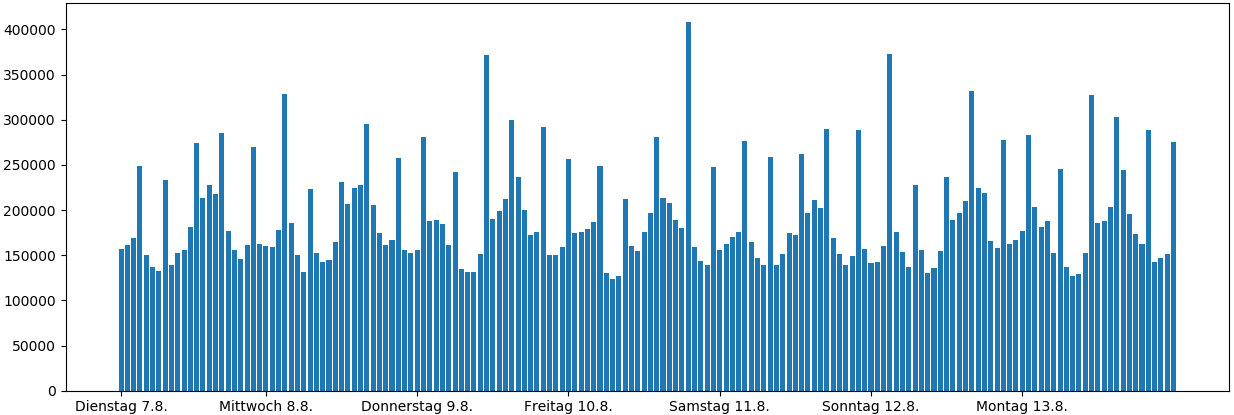
\includegraphics[scale=0.45]{Twitter-Daten.png}
 \caption{Anzahl Tupel pro Stunde.}
\end{figure}

\section{Systemaufbau}
Die Evaluation wurde auf dem internen OpenStack-Cluster des Instituts für Verteile und Parallele Systeme der Universität Stuttgart durchgeführt.
Für die Evaluation wurde ein Cluster aus vier virtuellen Maschinen aufgebaut.
Die Maschinen werden mit dem Betriebssystem Ubuntu 14.04 betrieben.
Drei der virtuellen Maschinen sind je mit 24 CPU-Kernen, 32 GB Arbeitsspeicher und 50 GB persistentem Speicher ausgestattet.
Diese Maschinen führen während der Evaluation die aktiven Tasks aus.
Die vierte Maschine wird als Steuer-Knoten genutzt und arbeitet mit 4 CPU-Kernen, 8 GB RAM sowie 10 GB persistentem Speicher.
Auf der vierten Maschine wird ausschließlich der Ablauf der Evaluation gesteuert.
Somit sind die Maschinen, die Tasks der Topologie ausführen, identisch.
Der Cluster wird über den Apache Aurora-Scheduler in der Version 0.13 gesteuert.
Der Scheduler von Aurora so wie die Steuerung des CEP befinden sich auf diesem Knoten.
Auf jedem der drei anderen Rechner ist die ausführende Instanz von Aurora ebenfalls in der Version 0.13 installiert.
Um die Arbeitspakete an die ausführenden Knoten auszuliefern, wird das verteile Dateisystem HDFS von Apache Hadoop in der Version 3.0.3 verwendet.
Der Adapter für das implementierte Framework wird ebenfalls auf diesem Rechner gestartet.
Zusätzlich benötigen die Systeme Apache Zookeeper um den verteilten Zustand zu speichern.
Dieser ist ebenfalls als Cluster über alle vier virtuellen Maschinen konfiguriert.

\section{Heron}
Für die Evaluation wurde das CEP-System Heron gewählt \cite{kulkarni_twitter_2015}.
Heron ist ein Nachfolger von Apache Storm.
Die Twitter Inc. entwickelte Heron als Nachfolger für den produktiv verwendeten Storm Cluster.
Sie entwickelten Heron als schnelleres und besser skalierendes System, da Storm den Anforderungen nicht mehr gerecht werden konnte \cite{kulkarni_twitter_2015}.
Heron wird von Twitter momentan als produktives System für die Analyse von Datenströmen eingesetzt.
Heron wurde für diese Evaluation aus zwei Gründen gewählt.
Einerseits ist aufgrund der produktiven Verwendung und aktiven Entwicklung bei Twitter ist davon auszugehen, dass das System aktuellen realen Anforderungen gerecht wird.
Zweitens wurde ein System gesucht, mit dem die Algorithmen möglichst unabhängig bewertet werden können.
Viele der in Kapitel ******** vorgestellten Algorithmen wurden auf Basis eines bestimmten CEP-Systems entwickelt.
Einige dieser CEP-Systeme sind Eigenentwicklungen oder erweiterte Frameworks auf bestehenden CEP-Systemen, die von den Autoren entwickelt werden.
Apache Storm wird ebenso, als eines der bekanntesten CEP-Systeme, oft als Basis für die Entwicklung von neuen Algorithmen verwendet.
Mit Heron können verschiedene Algorithmen getestet werden, ohne dass manche den Vorteil besitzen nativ für das CEP-Systems entwickelt worden zu sein.

Eine wichtige Neuerung bei Heron ist besonders hervorzuheben:
Das System bietet die Möglichkeit eine Topologie über eine autonome Strom-Regulation zu steuern.
Bei vielen anderen Systemen werden Tupel einfach verworfen, wenn die Kapazität eines Operators nicht mehr ausreicht.
Dieses Verhalten wird als sogenannter Lastabwurf bezeichnet.
Dies führt dazu, dass Tupel entweder verloren gehen oder von der Quelle erneut ausgegeben werden.
Wird ein Tupel neu ausgegeben, muss es alle Operatoren erneut durchqueren.
Diese Verhalten zusätzliche Last auf dem System verursachen und den Engpass noch verstärken.
Die neue Regulation in Heron wird aktiviert, wenn ein Operator die ankommende Menge von Tupel nicht mehr verarbeiten kann.
Dies wird von der Topologie erkannt und die Quellen werden daraufhin gestoppt.
Somit gelangen keine neuen Tupel mehr in die Topologie.
Der Stopp wird so lange aufrecht erhalten, bis der Operator wieder genügend Kapazität für neue Tupel geschaffen hat.

Diese Methode, den Datenstrom zu drosseln, verändert die Erkennung von Operatoren die Flaschenhälse bilden gänzlich.
Messwerte, auf die viele der in Kapitel 4 vorgestellten Algorithmen reagieren, verhalten sich anders.
Dies trifft auch für die beiden implementierten Algorithmen zu.
Diese gehen im Grundprinzip davon aus, dass bei einem Flaschenhals die Anzahl ankommender Tupel größer als die Anzahl abgearbeiteter Tupel ist.
Dieser Zustand kann aber nicht mehr auftreten, wenn die Quelle den Zufluss von neuen Tupeln automatisch stoppt.
Somit würde ein Operator gar nicht oder nur sehr schwach von den Algorithmen skaliert werden.
Deswegen wurde dieses Verhalten für die Evaluation der beiden Implementationen deaktiviert.

Die Evaluation wurde mit Heron unter der aktuellen Version 0.17.5 durchgeführt.
Die System-Parameter wurden im Standard belassen und nicht verändert.

\section{Topologie}

Für die Durchführung der Evaluation wurde eine eigene Topologie entwickelt.
Diese liest die von der Twitter API gesammelten Tupel aus und analysiert sie auf deren Eigenschaften.
Der logische Aufbau der Topologie ist in der Abbildung 10.2 dargestellt.
Ziel bei der Erstellung der Topologie war, dass es Operatoren mit unterschiedlich großen Lasten gibt.
Entweder wurde der Datenstrom durch eine Filteroperation für den Folgeoperator verkleinert oder die Operation des Operators rechenintensiv gestaltet.

\begin{figure}
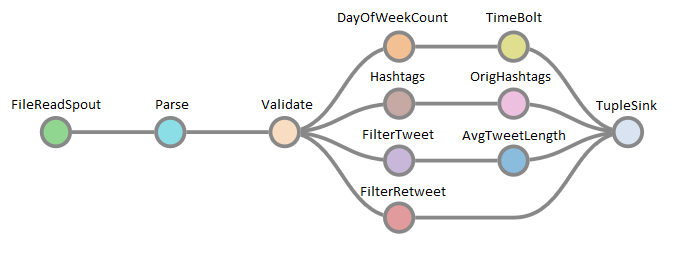
\includegraphics[scale=0.8]{Topologie.png}
\caption{Darstellung der logischen Topologie durch Heron UI.}
\end{figure}

Topologien in Heron besitzen Parameter, durch die der Entwickler das Verhalten beeinflussen kann.
Für nahezu alle Parameter definiert Heron einen Standardwert.
Im Folgenden werden die Parameter beschrieben, bei der die Evaluations-Topologie vom Standard abweicht.
Die Parameter sind in Tabelle 10.1 mit den zugewiesenen Werten aufgelistet.

Wie schon im vorherigen Kapitel beschrieben wurde die Regulation des Tupel-Stroms deaktiviert.
Die Topologie wurde so konfiguriert, dass jedes Tupel mindestens einmal erfolgreich verarbeitet werden muss.
Deshalb werden Tupel, die in der Folge eines Flaschenhalses verworfen werden, mehrfach von der Quelle ausgegeben.
Dies ist möglich, weil die Bestätigung von Tupel aktiviert wurde.
Dies bedeutet, dass jeder Operator die Bearbeitung des Tupels an die Quelle zurückmeldet.
Erst wenn alle Operatoren die Verarbeitung des Tupel bestätigen, wird das Tupel als bestätigt markiert.
Durch diesen Mechanismus ist es ebenfalls möglich die Latenz des Tupels zu bestimmen.
Die Quelle wurde so konfiguriert, dass ein Tupel, das innerhalb von einer Minute nicht erfolgreich verarbeitet wurde, ungültig ist und wiederholt werden muss.
Außerdem sendet die Quelle maximal 1.000.000 Tupel, ohne dass eines davon bestätigt wurde.
Das bedeutet, dass sich zu jedem Zeitpunkt maximal 1.000.000 Tupel zur Bearbeitung in der Topologie befinden.
Dieser Wert wurde bewusst sehr groß gewählt, um die Ausgabe von Tupeln nicht aufgrund von Flaschenhälsen in der Topologie zu verringern.
So ist sichergestellt, dass die Quelle dauerhaft in der Lage ist Tupel auszugeben, um den realistischen Arbeitsaufwand zu rekonstruieren.

\begin{table}
\caption{Parameter der Topologie}
\begin{tabular}{ll}
\hline
\textbf{Parameter} & \textbf{Wert} \\ \hline
TopologyDropTuplesUponBackpressure & True \\
TopologyReliabilityMode & ATLEAST\_ONCE \\
MessageTimeoutSecs & 60 \\
MaxSpoutPending & 1000000 \\
\hline
\end{tabular}
\end{table}

In der momentanen Version kann Heron die Operatoren nur skalieren, wenn die Tupel zufällig den Tasks der Operatoren zugewiesen werden.
Deswegen wurde diese Konfiguration für die Operatoren der Topologie gewählt.
Außerdem erhält jeder Folgeoperator immer alle ausgegebenen Tupel des Vorgängers.
Es gibt also keine selektive Weiterleitung.
Jedem Task wurde eine CPU, 1,25 GB RAM und 1,25 GB persistentem Speicher zugewiesen.
Die Topologie wurde mit der Java API von Heron entwickelt.
Diese erlaubt das definieren eigener Logik für die Quelle und die anderen Operatoren.
Im Folgenden werden die einzelnen Operatoren der Topologie beschrieben.

\subsection{Quelle}
Die Quelle ''FileReadSpout'' liest die gesammelten Daten von der Festplatte.
Dies geschieht Zeile für Zeile was jeweils einem Tupel entspricht.
Jedes erfasste Tupel besitzt einen Zeitstempel mit dem Zeitpunkt, an dem es erzeugt wurde.
Um den Twitter-Datenstrom realistisch nachzubilden wird dabei immer der Zeitstempel des eingelesenen Tupels überprüft.
Um die Topologie auszulasten ist der Datenstrom in der realen Geschwindigkeit, mit der er erfasst wurde, nicht ausreichend.
Deshalb wird die Zeit in der die Tupel verarbeitet wurden, auf eine kleineren Zeitraum komprimiert.
So bleibt die Struktur des Arbeitsaufwandes wie Lastspitzen und Lastabfall erhalten, wird aber in ein kürzeres Intervall geschoben um so insgesamt mehr Last zu erzeugen.
Das Ziel ist, dass in jeder realen Minute in der Evaluation 84 Minuten der aufgezeichneten Daten verarbeitet werden.
Somit werden in einer realen Stunde 84 Stunden der aufgezeichneten Daten.
Da eine Woche 168 Stunden hat dauert ein Durchlauf der Evaluation 2 Stunden.
Die Quelle wurde so implementiert, dass sie den Startzeitpunkt der Topologie sowie den Zeitstempel des ersten Tupels in Millisekunden speichert.
Während der Evaluation wird geprüft wie viele Millisekunden seit dem Start der Topologie vergangen sind.
Mit diesen Werten kann der maximale Zeitstempel errechnet werden, mit dem ein Tupel die Quelle verlassen darf.
Der maximale Zeitstempel errechnet sich aus der Differenz von aktuellem Zeitstempel und der Startzeit der Topologie die mit dem Faktor 84 multipliziert und zu dem Zeitstempel des ersten Tupels addiert wird.
Mit dieser Methode kann nicht garantiert werden, dass Tupel nicht langsamer ausgegeben werden, aber es wird verhindert, dass die Tupel schneller als der realistische Arbeitsaufwand ausgeben werden.
Die Leserate vom permanenten Speicher ist in der verwendeten Implementation wesentlich höher als die Rate des realistischen Arbeitsaufwandes, sodass eine langsamere Abgabe der Tupel unrealistisch ist.

\subsection{Andere Operatoren}

Um die folgenden Beschreibungen zu verstehen, sind folgende Erläuterungen notwendig.
Ein Retweet ist ein Statusupdate welches das Statusupdate eines anderen Nutzers ohne weitere Anmerkung weiterverbreitet.
Ein Antwort-Tweet ist ein Statusupdate, welches auf das Statusupdate eines anderen Nutzers antwortet.
Ein Tweet zitiert einen anderen Tweet wenn er ihn weiterverbreitet und Anmerkungen hinzufügt.

\begin{itemize}
\item{''Parse'': Dieser Operator liest das Tupel, das einen String, der ein JSON-Objekt beschreibt, und liest alle Daten des JSON Objektes aus. Anschließend werden ausgewählte Daten weiter gesendet. Löschanfragen für Statusmeldungen werden nicht weitergeleitet.}
\item{''Validate'': Dieser Operator prüft die Lesbarkeit der Daten und gibt sie auf der Standardausgabe aus.}
\item{''DayOfWeekCount'': Hier wird der Zeitstempel des Tupels in den Wochentag, an dem das Tupel erzeugt wurde, umgerechnet. Jedes Tupel erhöht den Zähler für den jeweiligen Tag.}
\item{''TimeBolt'': Dieser Operator gibt den genauen Datumstext für den Zeitstempel des Tupels auf der Standardausgabe aus.}
\item{''Hashtags'': Hier werden die Hashtags des Tweets ausgelesen. In einer Tabelle werden identische Hashtags gezählt.}
\item{''OrigHashtags'': Zählt ebenso Hashtags, allerdings nur für Original-Tweets eines Retweet oder Antwort-Tweet.}
\item{''FilterTweet'': Sendet nur Tweets weiter, die kein Retweet und kein Antwort-Tweet sind sowie keinen anderen Tweet zitieren.}
\item{''AvgTweetLength'': Berechnet die durchschnittliche Länge des verfassten Textes.}
\item{''FilterRetweet'': Sendet ausschließlich Retweets weiter.}
\item{''TupleSink'': Hat keine Operation außer die Tupel final zu bestätigen.}
\end{itemize}

\section{Ablauf}

In der Evaluation mussten die zuvor implementierten Algorithmen die Topologie steuern, während Sie die Tupel im Zeitfenster von zwei Stunden verarbeitet.
Für jeden der beiden Algorithmen von Lohrmann et al. und Zacheilas et al. wurden fünf Durchläufe gestartet.
Jeder Durchlauf startet mit dem aktivieren des Clusters.
Die Hauptsteuerung wurde so implementiert, dass sie alle fünf Minuten die Topologie durch den gewählten Algorithmus prüfen lässt.
Zuerst werden alle Messwerte des Graph-Modells mit den aktuellen Messwerten aus der Topologie aktualisiert.
Anschließend wurden die folgenden Daten zur Evaluation erfasst:
\begin{itemize}
\item{Minuten seit Beginn der Evaluation}
\item{Sekunden seit Beginn der Evaluation}
\item{Durchschnittliche Latenz der Tupel}
\item{Anzahl fehlgeschlagener Tupel}
\item{Anzahl bestätigter Tupel}
\item{Summe der Parallelisierungsgrade der Operatoren}
\end{itemize}
Die Anzahl der Minuten und Sekunden seit Beginn der Evaluation ist dabei um fünf Minuten verschoben, da der Erste Start der Hauptsteuerung erst zur ersten Prüfung erfolgt, nachdem die Topologie schon 5 Minuten aktiv ist.
Wenn alle Messwerte erfasst sind, startet der gewählte Algorithmus und die Topologie wird entsprechend der Empfehlung des Algorithmus skaliert.
Erst nachdem der Vorgang erfolgreich von Heron zurückmeldet wurde, beginnt das Zeitfenster von 5 Minuten bis zur nächsten Prüfung.

Während Heron die Topologie skaliert ist diese gestoppt, sodass während dieser Zeit keine neuen Tupel von der Quelle ausgegeben werden.
Dies wirkt sich offensichtlich auf die Zeitbeschränkung für die Tupel-Ausgabe der Quelle aus, da die Zeit, die seit Beginn der Evaluation vergangen ist, trotzdem weiter läuft.
Dies spiegelt auch das reale Verhalten wieder, da der reale Datenstrom ebenfalls zwischengespeichert werden müsste, solange die Topologie skaliert.
Während des Vorgangs löscht Heron außerdem alle Messdaten, da die alten Daten für den aktuellen Zustand der Topologie nicht mehr gültig sind.
Nachdem die Topologie wieder gestartet wurde, müssen sich die Zwischenspeicher vor und nach den Operatoren erst wieder mit Tupel füllen, um aussagekräftige Messwerte zu erhalten.
Deswegen ist es sinnvoll erst nach Abschluss des Vorgangs weitere fünf Minuten zu warten, bis die Messwerte im System wieder aussagekräftig sind.
Außerdem werden aus diesem Grund bei der Abfrage der Messwerte, die ebenfalls im Interval von fünf Minuten ausgelesen werden, nur die letzten drei Minuten aus dem CEP-System angefordert.
Dies bedeutet, dass die Messwerte der ersten zwei Minuten, nachdem die Topologie skaliert wurde, weder für die Berechnung des Parallelisierungsgrades noch für die Ergebnisse der Evaluation verwendet wurden.
Die Evaluation stoppt sobald alle Tupel verarbeitet wurden.

\section{Parametrisierung der Algorithmen}

Für die Durchführung der Evaluation mussten die beschriebenen Parameter der Algorithmen definiert werden.
Das GraphModell war so konfiguriert, dass der minimale Parallelisierungsgrad eins und der maximale zehn beträgt.
Da jeder Task eines Operators eine CPU, und 1,25 RAM verbraucht, konnte der maximale Parallelisierungsgrad nicht höher als 10 gesetzt werden.

Für die Evaluation wurden für den Warteschlangen-Algorithmus die in der Tabelle 10.3 gelisteten Parameter gewählt.
Wie im Original von Lohrmann et al. wurde die Erkennung eines Flaschenhalses ab einer Auslastung von 100\% gesetzt.
Der Koeffizient für adaptives Batching wurde auf null gesetzt, da Heron diese Methode nicht verwendet.
Der Parameter bestimmt ohnehin nur den Anteil der maximalen Latenz des Pfades, der für adaptives Batching reserviert ist.
So kann dieser Anteil auch direkt bei der Angabe der maximalen Latenz berücksichtigt werden, wenn der Parameter auf null steht.
Die Schrittweite des Algorithmus wurde ebenfalls wie im Original auf eins gesetzt.
Die Verwendung des Koeffizienten e wurde deaktiviert, da die gemessene Latenz im Vergleich zu der vom Algorithmus berechneten Latenz sehr hoch war.
Dies hätte wie in Kapitel 8.2.4 beschrieben dazu geführt, dass der Algorithmus sehr hohe Parallelisierungsgrade vorgeschlagen hätte.
Dies hätte in Kombination mit dem maximalen Parallelisierungsgrad von zehn zur Folge gehabt, dass die Topologie während der Evaluation konstant maximal skaliert ist und nie angepasst wird.

\begin{table}
\caption{Parameter für den Warteschlangenalgorithmus}
\centering
\begin{tabular}{ll}
\hline
\textbf{Parameter} & \textbf{Wert} \\ \hline
BOTTLENECK\_THRESHOLD & 1.0 \\
ADAPTIVE\_BATCHING\_COEFFICIENT & 0.0 \\
DELTA\_STEP\_SIZE & 1 \\
USE\_LATENCY\_ADAPTION & False\\
\hline
\end{tabular}
\end{table}

Für den Algorithmus, der Regression zur Vorhersage verwendet wurden die in Tabelle 10.4 gezeigte Parametrisierung gewählt.
Die Trainingdaten für den Algorithmus wurden während der Evaluation des Lohrmann Algorithmus gesammelt.
Alle fünf Minuten, in denen die neuen Metriken aus dem System abgerufen wurden, wurden für jeden Operator die Anzahl eingegangener und ausgegangener Tupel der letzten drei Minuten mit Zeitstempel versehen und gespeichert.
Da die aus der Topologie bezogenen Messdaten vom aktuellen Zustand der Topologie und nicht von den verwendeten Twitter-Daten abhängen, sind auch Fehler reflektiert, die vom Algorithmus von Lohrmann et al. gemacht werden.
Somit ist garantiert, dass die verwendeten Trainingsdaten das Vorhersage-Modell nicht speziell für den vorliegenden Twitter-Datensatz übertrainiert wird.

Die Hyperparameter wurden für die Evaluation nicht mathematisch optimiert.
Sie wurden lediglich so gewählt, dass die Regression Vorhersagen im richtigen Größenbereich trifft.
Dazu wurden die Zeitstempel sehr schwach gewichtet.
Die Zeit, die seit der Evaluation vergangen ist, wurde stark gewichtet, da sie einen größeren Zusammenhang mit dem Zustand der Topolgie aufweiste als der Zeitstempel.
Da das Modell für eingehende Tupel nur auf den beiden Dimensionen Zeitstempel und vergangene Zeit beruht, muss die vergangene Zeit stark gewichtet werden um zu verhindern, dass der Zeitstempel das Modell verfälscht.
Für die Vorhersage der ausgehenden Tupel wurde die Gewichtung des Parallelisierungsgrad so gewählt, dass er sich in etwa gleich wie die vergangene Zeit auf die Korrelation auswirkt.
Wie in Kapitel 9.2.2 erwähnt besitzen der Parallelisierungsgrad und die Zeit, die seit der Evaluation vergangen ist, verschiedene Größenordnungen.
In der Evaluation bewegen sich Parallelisierungsgrade im Einerbereich währen die Zeit bis zu 7200 steigt.
Diese Tatsache wird durch den gewählten Wert des Hyperparameters ausgeglichen.

Die Kostenfunktion wurde für alle Kostenfaktoren mit eins initialisiert.
Dies fördert die Flexibilität der Topologie, da die Kosten, die Topologie zu ändern, und die Kosten pro verwendeten Task sehr gering sind.
Die Anzahl verpasster Tupel kann jedoch schnell 1000 übersteigen, sodass die Kosten für verpasste Tupel ausschlaggebend für den kürzesten Pfad im Graphen der Zustandsübergänge sind.
Die Vorhersagen wurden für Zeitfenster von fünf Minuten getroffen, um dem gleich dem Intervall zu sein, in dem die Topologie geprüft wird.
Es wurden jede Runde Vorhersagen für sechs Zeitfenster getroffen, sodass immer Zustandsübergänge für die nächsten 30 Minuten berücksichtigt wurden.

\begin{table}
\caption{Parameter für den Algorithmus mit Regression} 
\centering
\begin{tabular}{ll}
\hline
\textbf{Parameter} & \textbf{Wert} \\ \hline
SIGMA\_INPUT & 1.0 \\
LAMBDA\_INPUT & (1.0, 10000.0) \\
SIGMA\_OUTPUT & 1.0 \\
LAMBDA\_OUTPUT & (1.0, 10000.0 10.0) \\
Kostenfunktion & (1.0, 1.0, 1.0) \\
Abstand Zeitfenster & 300 \\
Anzahl Zeitfenster & 6 \\
\hline
\end{tabular}
\end{table}

\section{Ergebnisse}




Letzte wird nie parallelisiert bei zacheilas
Lohrmann hat vorteil, weil 2 Minuten nicht gemessen werden
Zacheilas bewegt sich im bekannten gefilde
Selten max erreiht, Ressourcen kein problem

